\chapter{Experiments}

\section{Datasets}
\label{sec:exp-datasets}
\subsection{MPII Human Pose}
\label{sec:exp-mpii}

\subsection{Penn Action}
\label{sec:exp-penn}

\subsection{JHMDB}
\label{sec:exp-jhmdb}


\section{Evaluation Metrics}
\subsection{Accuracy}

\subsection{Precision and Recall}

\subsection{F1-Score}


\section{Experimental Results}
\subsection{Accuracy of Soft-argmax function}
For evaluating the accuracy of the Soft-argmax function, we performed two experiments.
For both experiments, an estimated coordinate $(x_{est},y_{est})$ was considered to be correct in comparison to the ground truth coordinate $(x_{gt}, y_{gt}$ if both $\lvert x_{est} - x_{gt} \rvert \leq 2$ and $\lvert y_{est} - y_{gt} \rvert \leq 2$, allowing for a $2$ pixel discrepancy between prediction and ground truth.
The reason for using a threshold of $2$ pixels was that the output of the Soft-argmax function are fractions of width and height with $(x_{frac}, y_{frac}) \in [0,1]$.
To compute the image coordinate, a multiplication with the width and height of the input image as well as a rounding step is necessary, possibly introducing rounding errors.

First, synthetic images of size $256 \times 256$ pixels were created, since this is the size of the input images to the network after preprocessing.
At each $x,y$ position, a two-dimensional gaussian with mean $(x,y)$ and covariance $v$ was placed.
Afterwards, the expectations were computed using the Soft-argmax function and compared to the ground truth mean value.
Performing this for each pixel coordinate and different covariances $v$, it was observed that the Soft-argmax function accurately regressed the true expectation for small covariances.
As the covariance increases, the accuracy decreases, especially around the borders.
See \fref{fig:softargmax_variance_test} for a visualization, where violett pixels indicate a wrong prediction and yellow pixels indicate a correct prediction.
Second, synthetic joint heatmaps were generated by placing gaussians at the position of the ground truth label coordinates of a subset of the MPII dataset and the distance between the computed coordinates and ground truth coordinate was computed with different covariance values $v$.
The experiment was conducted on $100$ random images from the MPII dataset.
See \tref{tab:softargmax_numeric_eval} for the mean accuracies achieved for covariances $v \in \{1, 2, 5, 10, 20, 50 \}$.
%TODO: Talk about the results

\begin{table}[]
    \centering
    \scalebox{0.90}{%
    \begin{tabular}{|l|l|l|l|l|l|}
    \hline
    \textbf{$v=1$} & \textbf{$v=2$} & \textbf{$v=5$} & \textbf{$v=10$} & \textbf{$v=20$} & \textbf{$v=50$} \\ \hline
    TODO & TODO & TODO & TODO & TODO & TODO \\ \hline 
    \end{tabular}}
    \caption{Mean average accuracy of Soft-argmax when detecting ground truth coordinates from synthetic joint heatmaps.} %TODO: Talk about results here too
    \label{tab:softargmax_numeric_eval}
\end{table}

%TODO: Small evaluation of the results of both experiments
This suggests that the Soft-argmax function requires that the heatmap used is highly accurate by itself and that the joints are not too near to the image border.

\begin{figure}[htb!]
    \centering
    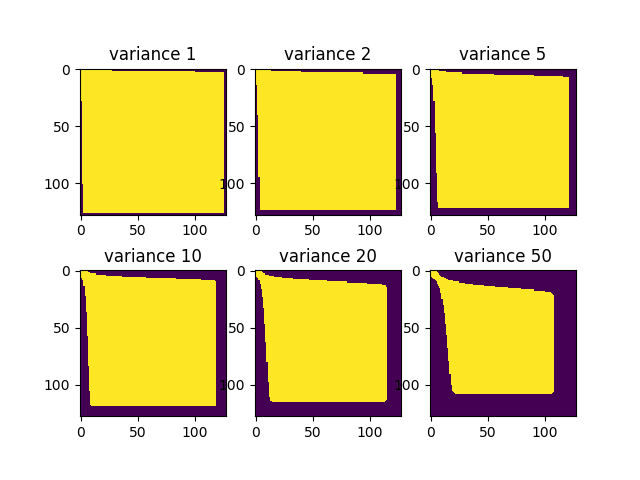
\includegraphics[width=0.7\textwidth]{softargmax_variance_test.png}
    \caption{Evaluation of the accuracy of the Soft-argmax function using synthetic data. Yellow pixels $i,j$ indicate where the Soft-argmax function correctly regressed the peak of the gaussian with mean value $i,j$, while violett indicates wrong predictions. Notice that the accuracy decreases when approaching the border of the image and when the covariance is increasing. }
    \label{fig:softargmax_variance_test}
\end{figure}

\subsection{Replication of Original Work}
\label{sec:exp-replication}

\subsection{Results on JHMDB Dataset}

\subsection{Effect of Combining Loss Functions}

\subsection{Effect of Using Different Representations of Pose}
\label{sec:different_pose_representation_experiment}

